%---------- Segundo Capitulo ----------
\chapter{Fundamentação Teórica}
\section{Autenticação}
Em sistemas computacionais em que a identificação e autenticação do usuário são premissas na segurança de transações e processos, é interessante manter mecanismos que ofereçam aos usuários, meios confiáveis no estabelecimento dessas conexões.
\begin{citacao}
Durante as primeiras décadas de sua existência, as redes de computadores foram usadas principalmente por pesquisadores universitários, com a finalidade de enviar mensagens de correio eletrônico, e também por funcionários de empresas, para compartilhar impressoras. Sob essas condições, a segurança nunca precisou de maiores cuidados. Porém, como milhões de cidadãos comuns atualmente estão usando as redes para executar operações bancárias, fazer compras e arquivar sua devolução de impostos, a segurança das redes está despontando no horizonte como um problema potencial.\cite{tanenbaum2003redes}
\end{citacao}
Frequentemente para utilizar algum recurso computacional são utilizadas três técnicas de autenticação de usuários:
\begin{enumerate}[(a)]
\item algo que o usuário sabe – uma senha, a resposta para alguma pergunta ou reconhecimento de algum padrão;
\item algo que o usuário tem – um cartão magnético, um crachá ou um token de segurança;
\item como o usuário é – baseado em características biométricas.
\end{enumerate}

As técnicas (a) e (b) podem ser passíveis de fraude, tendo em vista que alguém possuindo tais informações/objetos pode facilmente conseguir acesso ao sistema como se fosse o verdadeiro usuário. Além disso, esses fatores necessitam da interação direta do usuário, isto é, o usuário deve informar estes dados para realizar a autenticação, geralmente via dispositivos de entrada comuns, como microfone, tela ou teclado.

\begin{figure}[!htb]
	\centering
	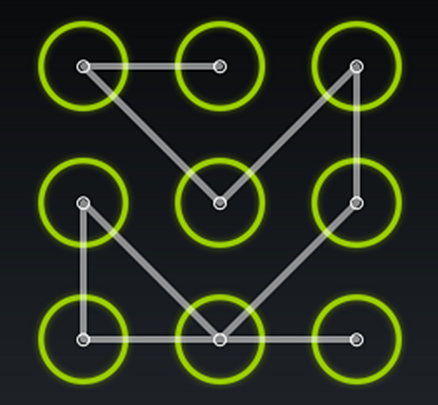
\includegraphics[width=0.2\textwidth]{trace.png} % <- formatos PNG, JPG e PDF
	\small
	\caption[Uso de senha por reconhecimento de padrão]{Uso de senha por reconhecimento de padrão nos \textit{smartphones} Android}
	\label{fig:trace}
\end{figure}

\subsection{O uso de senhas}
Mesmo a autênticação através do uso de senhas ser o alvo de várias formas de ataque, ela é uma das mais empregadas como meio de assegurar a privacidade de sistemas.
\begin{citacao}
Algumas das formas como a sua senha pode ser descoberta são:
\begin{enumerate}
\item ao ser usada em computadores infectados. Muitos códigos maliciosos, ao infectar um computador, armazenam as teclas digitadas (inclusive senhas), espionam o teclado pela webcam (caso você possua uma e ela esteja apontada para o teclado) e gravam a posição da tela onde o mouse foi clicado;
\item ao ser usada em sites falsos. Ao digitar a sua senha em um site falso, achando que está no site verdadeiro, um atacante pode armazená-la e, posteriormente, usá-la para acessar o site verdadeiro e realizar operações em seu nome;
\item ao ser capturada enquanto trafega na rede, sem estar criptografada;
\item com o uso de técnicas de engenharia social, como forma a persuadi-lo a entregá-la voluntariamente;
\item pela observação da movimentação dos seus dedos no teclado ou dos cliques do mouse em teclados virtuais.
\cite{Cert2016}
\end{enumerate}
\end{citacao}

Para melhorar a eficiência no uso de senhas muitas organizações adotam políticas de segurança que impõem regras no uso das mesmas, além disso, criam mecanismos para que as senhas tenham um determinado formato, utilizam algum algorítmo de criptografia, senhas expiram em um determinado tempo, tudo para tentar aumentar a segurança de seus sistemas.

\begin{table}[!htb]
  	\centering
	\label{tab:ISO17}
	\begin{tabular}{|*3{c|}} \hline
		\multicolumn{3}{|c|}{A.11.2 Gerenciamento de acesso do usuário}\\ \hline
		A.11.2.1 & Registro de usuário & \vtop{\hbox{\strut Controle}\hbox{\strut Deve existir um procedimento formal de registro e}\hbox{\strut cancelamento de usuário para garantir e revogar }\hbox{\strut acessos em todos os sistemas de informação}\hbox{\strut e serviços.}} \\ \hline
		A.11.2.3 & \vtop{\hbox{\strut Gerenciamento de}\hbox{\strut senha do usuário}} & \vtop{\hbox{\strut Controle}\hbox{\strut A concessão de senhas deve ser controlada}\hbox{\strut por meio de um processo de gerenciamento formal.}} \\ \hline
	\end{tabular}
	\caption[Objetivos de controle e controles na ABNT NBR ISO/IEC 17799:2005]{Objetivos de controle e controles apresentados na ABNT NBR ISO/IEC 17799:2005 \cite{nbr27001}}
\end{table}